% Each row: /contrasts three_seed_arithmetic_mean audited_disparity gain.normalized;
% interval: /participant_cluster_bootstrap/contrasts with key
% [contrast_id, "three_seed_mean", "disparity_gain:" + field], percentile_95.normalized.
% Rounded to six decimals for display; the immutable JSON retains full precision.
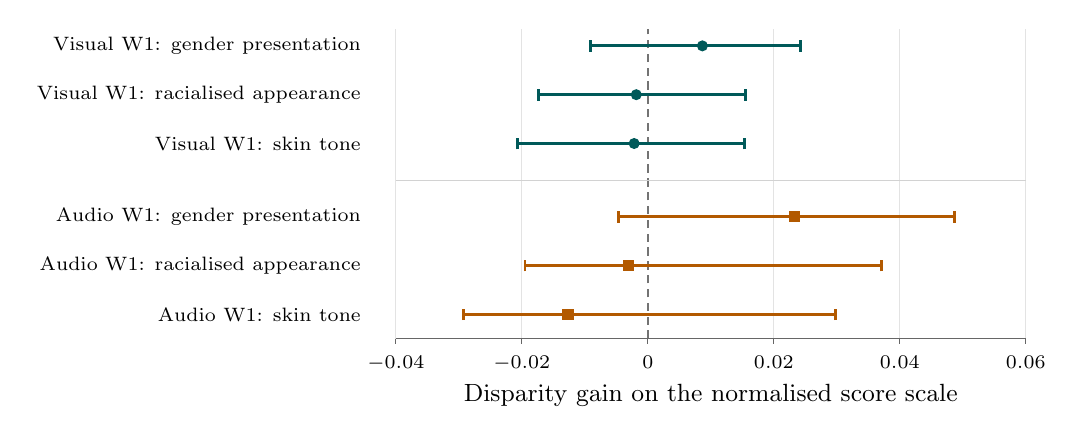
\begin{tikzpicture}[x=80cm,y=0.62cm]
  \foreach \x in {-0.04,-0.02,0.02,0.04,0.06} {
    \draw[gray!22] (\x,0.0) -- (\x,6.35);
  }
  \draw[black!55,densely dashed,line width=0.8pt] (0,0.0) -- (0,6.35);
  \draw[black!60] (-0.04,0.0) -- (0.06,0.0);
  \draw[gray!35] (-0.04,3.25) -- (0.06,3.25);

  \foreach \x/\label in {-0.04/$-0.04$,-0.02/$-0.02$,0/$0$,0.02/$0.02$,0.04/$0.04$,0.06/$0.06$} {
    \draw[black!60] (\x,0.0) -- (\x,-0.10);
    \node[font=\scriptsize,anchor=north] at (\x,-0.16) {\label};
  }
  \node[font=\small,anchor=north] at (0.01,-0.72)
    {Disparity gain on the normalised score scale};

  \node[font=\scriptsize,anchor=east] at (-0.044,6) {Visual W1: gender presentation};
  \node[font=\scriptsize,anchor=east] at (-0.044,5) {Visual W1: racialised appearance};
  \node[font=\scriptsize,anchor=east] at (-0.044,4) {Visual W1: skin tone};
  \node[font=\scriptsize,anchor=east] at (-0.044,2.5) {Audio W1: gender presentation};
  \node[font=\scriptsize,anchor=east] at (-0.044,1.5) {Audio W1: racialised appearance};
  \node[font=\scriptsize,anchor=east] at (-0.044,0.5) {Audio W1: skin tone};

  % Visual W1 versus same-seed ERM: pointwise 95% participant-cluster intervals.
  \draw[teal!70!black,line width=1pt] (-0.009153,6) -- (0.024242,6);
  \draw[teal!70!black,line width=1pt] (-0.009153,5.88) -- (-0.009153,6.12);
  \draw[teal!70!black,line width=1pt] (0.024242,5.88) -- (0.024242,6.12);
  \fill[teal!70!black] (0.008671,6) circle[radius=2pt];

  \draw[teal!70!black,line width=1pt] (-0.017332,5) -- (0.015458,5);
  \draw[teal!70!black,line width=1pt] (-0.017332,4.88) -- (-0.017332,5.12);
  \draw[teal!70!black,line width=1pt] (0.015458,4.88) -- (0.015458,5.12);
  \fill[teal!70!black] (-0.001826,5) circle[radius=2pt];

  \draw[teal!70!black,line width=1pt] (-0.020646,4) -- (0.015386,4);
  \draw[teal!70!black,line width=1pt] (-0.020646,3.88) -- (-0.020646,4.12);
  \draw[teal!70!black,line width=1pt] (0.015386,3.88) -- (0.015386,4.12);
  \fill[teal!70!black] (-0.002168,4) circle[radius=2pt];

  % Interview-audio W1 versus same-seed ERM, plotted with square markers.
  \draw[orange!70!black,line width=1pt] (-0.004588,2.5) -- (0.048720,2.5);
  \draw[orange!70!black,line width=1pt] (-0.004588,2.38) -- (-0.004588,2.62);
  \draw[orange!70!black,line width=1pt] (0.048720,2.38) -- (0.048720,2.62);
  \node[rectangle,fill=orange!70!black,minimum size=4pt,inner sep=0pt] at (0.023337,2.5) {};

  \draw[orange!70!black,line width=1pt] (-0.019508,1.5) -- (0.037087,1.5);
  \draw[orange!70!black,line width=1pt] (-0.019508,1.38) -- (-0.019508,1.62);
  \draw[orange!70!black,line width=1pt] (0.037087,1.38) -- (0.037087,1.62);
  \node[rectangle,fill=orange!70!black,minimum size=4pt,inner sep=0pt] at (-0.003113,1.5) {};

  \draw[orange!70!black,line width=1pt] (-0.029259,0.5) -- (0.029783,0.5);
  \draw[orange!70!black,line width=1pt] (-0.029259,0.38) -- (-0.029259,0.62);
  \draw[orange!70!black,line width=1pt] (0.029783,0.38) -- (0.029783,0.62);
  \node[rectangle,fill=orange!70!black,minimum size=4pt,inner sep=0pt] at (-0.012670,0.5) {};
\end{tikzpicture}
